% !TeX spellcheck = en_GB
\documentclass[12pt]{article}    
\usepackage{ucs} 
\usepackage[utf8x]{inputenc}
\usepackage[russian]{babel}  
\usepackage{float}
\title{Лабораторная работа №3\\}
\author{Хафизов Фанис}
\usepackage[pdftex]{graphicx}

\begin{document}
	\begin{figure}
		\centering
		
\includegraphics[width=0.3\linewidth]{logo}
	\end{figure}
	\maketitle
	\newpage
	\section{Цель работы}
	Изучение явлений, связанных с распространением звуковых волн в воздушной среде.
	\section{Схема установки}
	Лабораторная установка представляет собой трубу из прозрачного пластика,
	смонтированную на специальной подставке. К верхнему концу трубы пристыкован динамик, излучающий звуковую волну, распространяющуюся внутри трубы.\\
	К приборам и принадлежностям относятся датчик звука с двумя микрофонами внутри трубы и компьютер с необходимым программным обеспечением и соединительный кабель. Один из микрофонов закреплен неподвижно, а другой перемещается вдоль трубы.
	\section{Порядок действий}
	1)Соберем экспериментальную установку.\\
	2)Установим частоту колебаний $\nu=$1500Гц.\\
	3)Включим генератор колебаний и начнем передвигать подвижный микрофон, при этом записывая значения смещения микрофона, при которых фаза его колебаний будут совпадать с фазой колебаний неподвижного микрофона.\\
	4)Воспользовавшись средним значением смещения микрофона, и значением частоты, на которой работатет генератор, рассчитаем скорость звуковой волны.\\
	5)Теперь будем передвигать повижный микрофон и записывать разницу во времени между характерными точками на графиках. Также будем записывать смещение подвижного микрофона.\\
	6)Построим график зависимости смещения микрофона от времени по точкам из п.5 и найдем скорость звука как угловой коэффициент наклона.
	\section{Таблицы данных и графики}
	\begin{table}[H]
		\begin{tabular}{|l|}
			\hline
			l, см \\ \hline
			0,0   \\ \hline
			23,5  \\ \hline
			45,0  \\ \hline
			69,5  \\ \hline
		\end{tabular}
		\caption{Значения смещений микрофона, при которых фазы микрофонов совпадают}
	\end{table}
	\begin{table}[H]
		\begin{tabular}{|l|l|}
			\hline
			l, см & t, мс \\ \hline
			0     & 0,00  \\ \hline
			15    & 0,33  \\ \hline
			30    & 0,71  \\ \hline
			45    & 1,31  \\ \hline
			60    & 1,64  \\ \hline
			75    & 2,04  \\ \hline
		\end{tabular}
		\caption{Зависимость времени от смещения микрофона}
	\end{table}
	\begin{figure}[H]
		\centering
		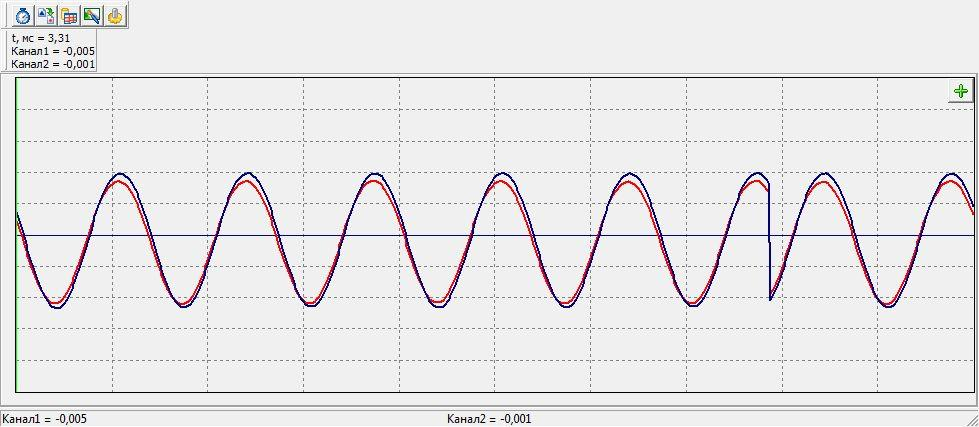
\includegraphics[scale=0.7]{graph1}
		\caption{Совпадение фаз колебаний на 2 микрофонах}
	\end{figure}
	\begin{figure}[H]
		\centering
		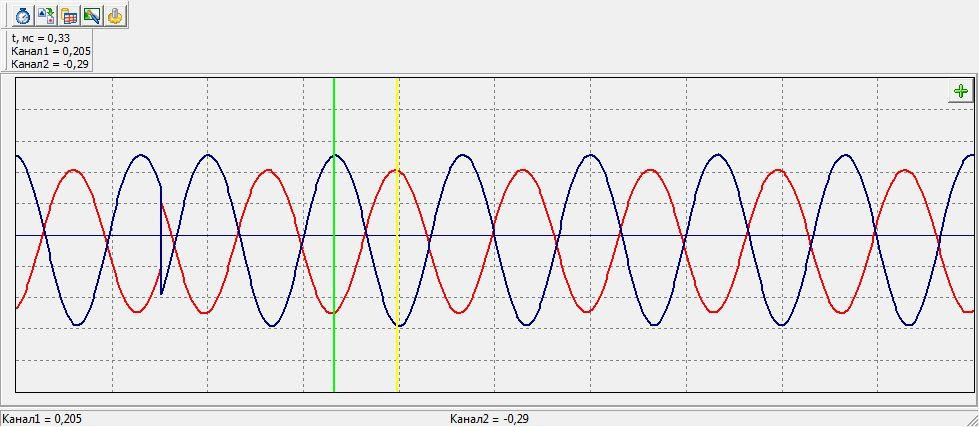
\includegraphics[scale=0.7]{graph2}
		\caption{Разница между колебаниями при смещении подвижного микрофона}
	\end{figure}
	\begin{figure}[H]
		\centering
		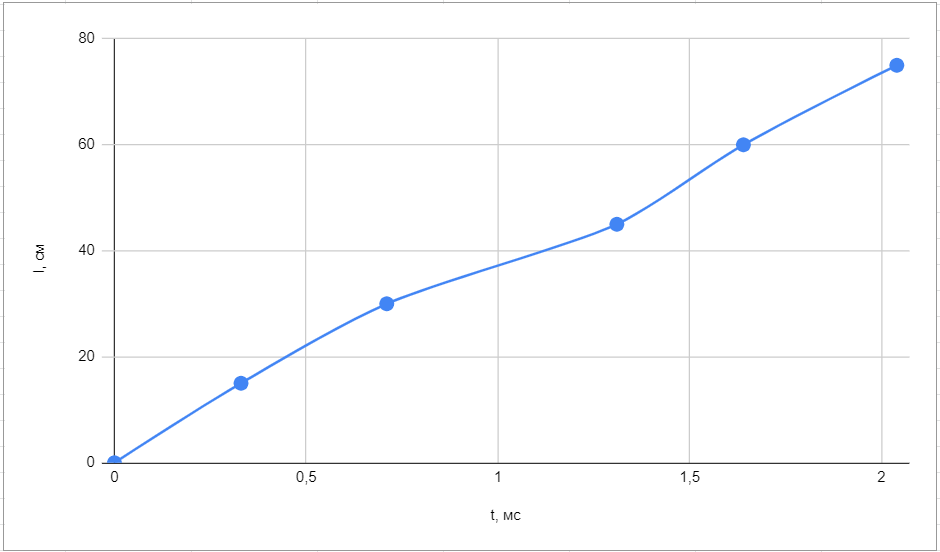
\includegraphics[scale=0.7]{graph3}
		\caption{График зависимости смещения подвижного микрофона от разницы времен фиксации сигнала микрофонами}
	\end{figure}
	\section{Расчеты}
	$\displaystyle v_{th}=\sqrt{\frac{\gamma RT}{\mu}}=\sqrt{\frac{1{,}4\cdot8{,}31\cdot298}{0{,}029}}=345{,}8$ м/с\\
	$\displaystyle\overline{\Delta l}=\frac{\sum\limits_{i=1}^{3}l_{i+1} - l_i}{3}=69{,}5/3=23{,}17$ см\\
	$\displaystyle v_{pr1}=\nu\cdot\overline{\Delta l}=1500\cdot0{,}2317=347{,}5$ м/с\\
	$v_{pr2}=354$ м/с\\
	$\displaystyle\Delta(\Delta l)=2\sqrt{\frac{\sum \limits_{i=1}^{3} (\Delta l_i-\overline{\Delta l})^2}{3}}=2{,}5$ см\\
	$\displaystyle\varepsilon_{\Delta l}=\frac{\Delta(\Delta l)}{\overline{\Delta l}}=2{,}5/23{,}17=11\%$\\
	$\displaystyle\varepsilon_{v1}=\varepsilon_{\Delta l}=11\%$\\
	$\displaystyle\Delta v_{pr1}=\varepsilon_{v1}\cdot v_{pr1}=38{,}3$ м/с\\
	$\displaystyle\Delta v_{pr2}=2\sqrt{\frac{\sum \limits_{i=1}^{5} (\frac{\Delta l_i}{\Delta t_i}-\overline{\frac{\Delta l}{\Delta t}})^2}{5}}=150$ м/с\\
	$\varepsilon_{v2}=\frac{\Delta v_{pr2}}{v_{pr2}}=150/354=43\%$
	\section{Результаты}
	$\displaystyle v_{th}=345{,}8$ м/с\\
	$\displaystyle v_{pr1}=(347{,}5\pm38{,}3)$ м/с\\
	$v_{pr2}=(354\pm150)$ м/с\\
	$\delta_v1=11\%$\\
	$\delta_v2=43\%$\\
	\section{Выводы}
	Полученные в ходе экспериментов результаты близки к теоретическому значению, однако, величина относительной погрешности достаточно велика. В первом эксперименте это можно объяснить малым количеством измерений, из-за недостаточно большной длиной трубы. Во втором же случае был выбран плохой метод для оценки погрешности, который все же не отразился на численном ответе. Для уменьшения погрешности я бы предложил использовать микрофоны и динамик лучшего качества, а также увеличить длину трубы. 
\end{document}